\section{Results}

Using the $Beta\_SSE$ score, we construct a timeseries of the level of market efficiency as seen in Figure~\ref{fig:sp_500_SSE_beta_ts}.
We shade in grey the recession periods as defined by NBER based Recession Indicators \citep{usrec}
\begin{figure}[h!]
    \centering
    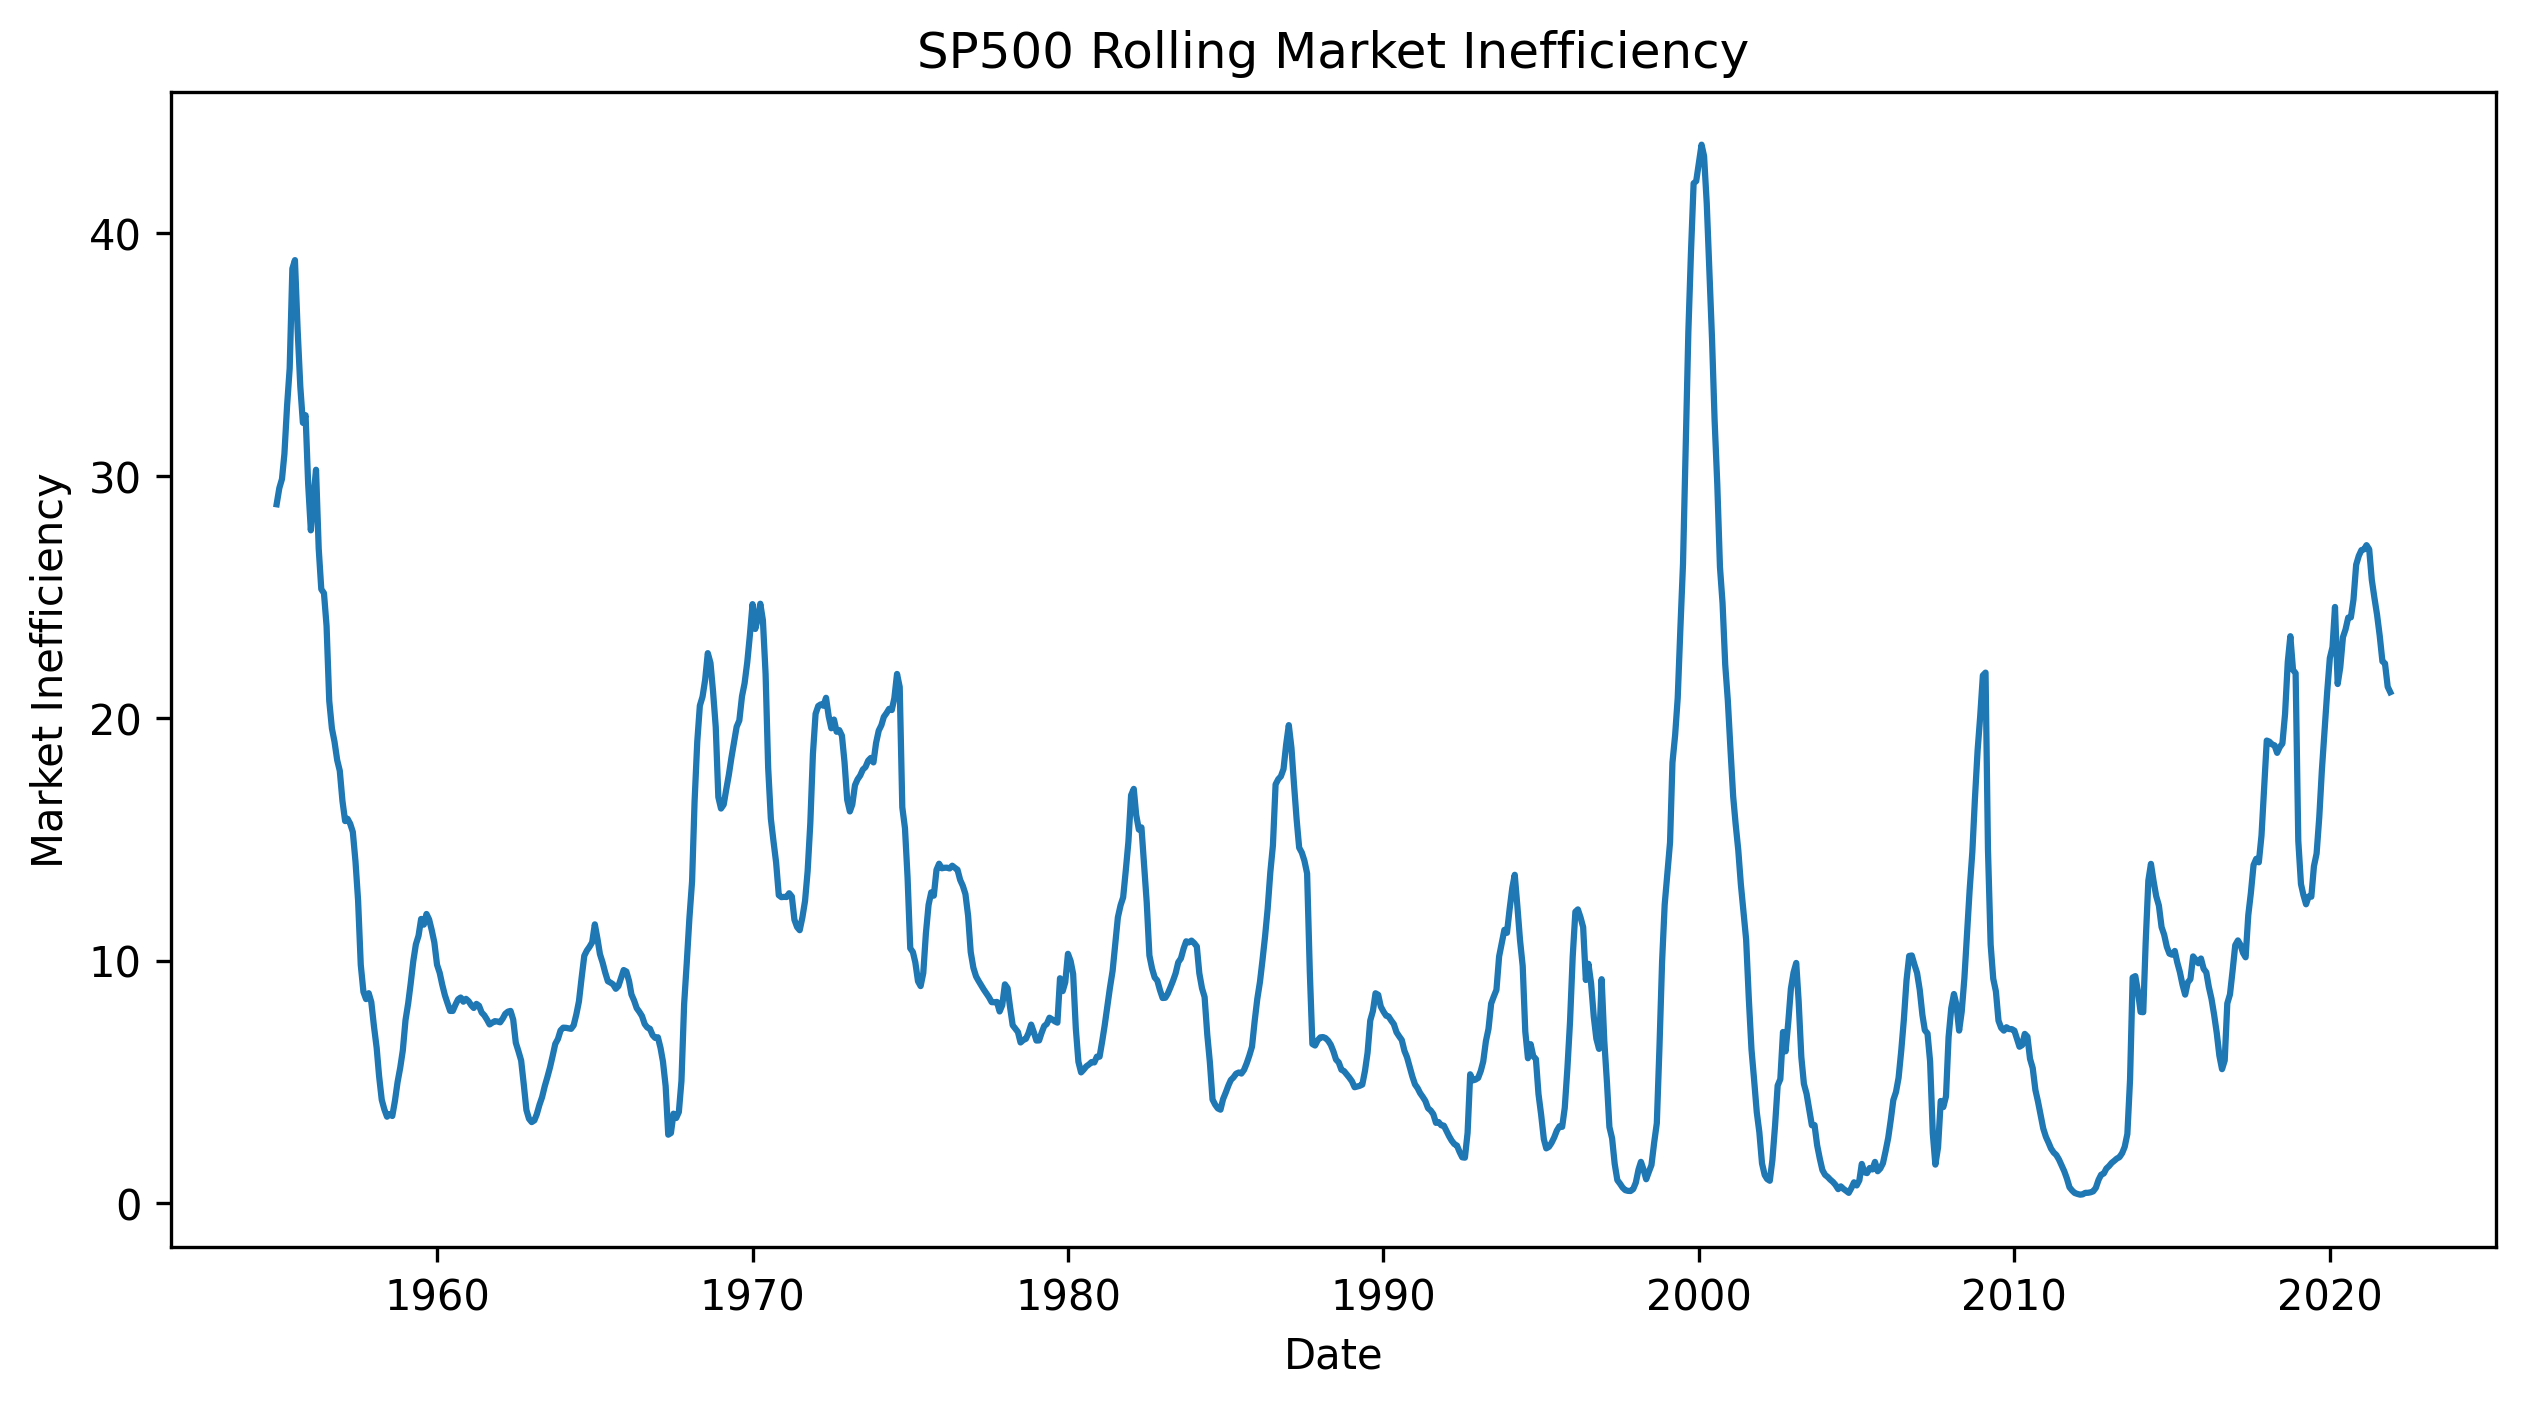
\includegraphics[width=0.9\textwidth]{../figs/SP500 Rolling Market Inefficiency.png}
    \caption{The $Beta\_SSE$ score timeseries of the SP500 (1950 - 2024)}
    \label{fig:sp_500_SSE_beta_ts}
\end{figure}

We see the market is inefficient around the dot-com bubble, the 2008 financial crisis, and the COVID-19 pandemic, which is in line with our expectations.
We can visually asses that the market is not uniformly efficient. Instead, it goes through periods of higher inefficiency followed by reversion to efficiency.
We also see that the market has been increasingly inefficient in the last decade, which is in line with \citet{asness_2024}.

Empirically we can test the mean reversion through an Augmented Dickey-Fuller test \citep{cheung1995lag} on the $Beta\_SSE$ timeseries, which is significant at the 0.1\% level.

Figure~\ref{value_spread_beta_sse} shows the value spread and the $Beta\_SSE$ score timeseries. We see visually that the two are cointegrated, which we test with
the Engle-Granger two-step cointegration test, which is significant at the 0.5\% level.

\begin{figure}[h!]
    \centering
    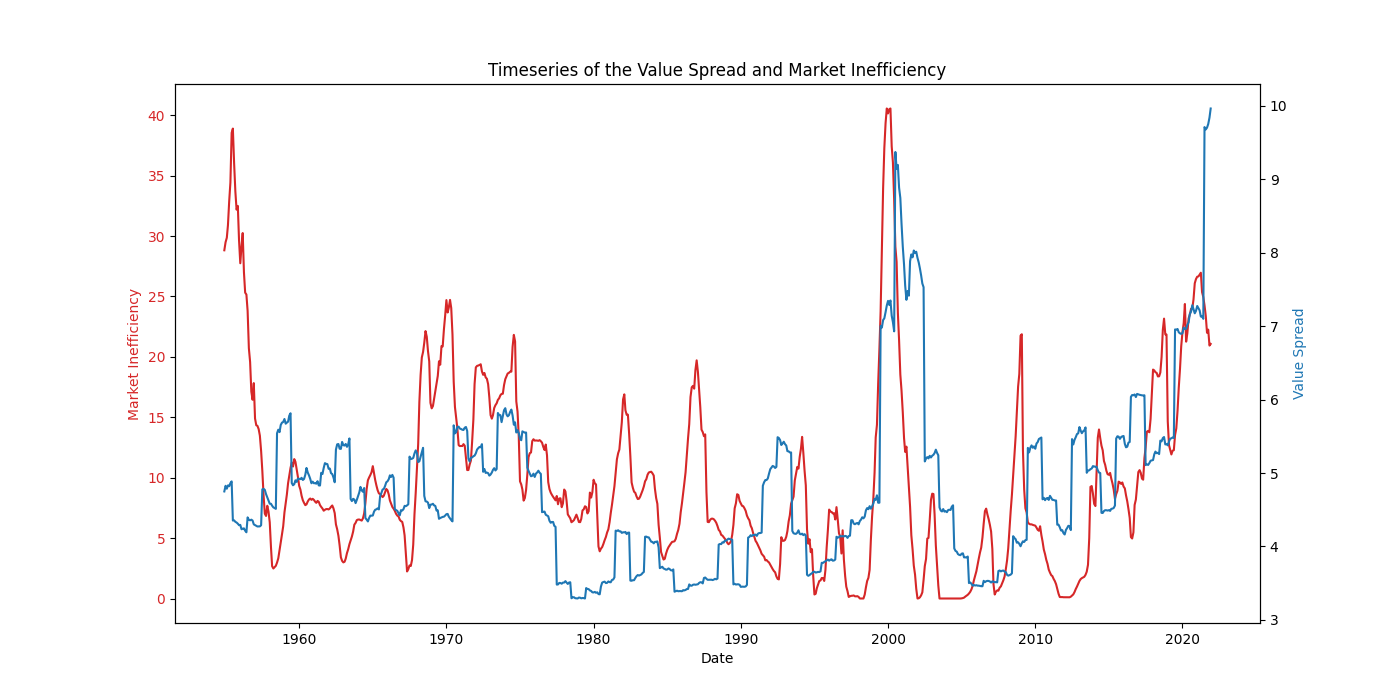
\includegraphics[width=0.9\textwidth]{../figs/Value Spread and Market Inefficiency.png}
    \caption{The value spread and $Beta\_SSE$ score timeseries of the SP500 (1950 - 2024)}
    \label{value_spread_beta_sse}
\end{figure}